%! TEX root = ../main.tex 

\chapter{The Pierre Auger Observatory}
\label{chap:pierre-auger-observatory}

The \PAO is the largest scientific experiment in the world, spanning an area of
roughly \SI{3000}{\kilo\meter\squared}. It consists of an array of 1660 \WCDs, 
which form the \SD, and 27 fluorescence telescopes, that comprise the \FD. The
simultaneous detection of \CR-artifacts in the air and on ground via this hybrid
approach offers a unique possibility to observe \UHECRs at the tail-end of the 
\CR energy spectrum.

\section{Project History and Future}
\label{sec:project-history-and-future}

\subsection{Science Goals and Achievements}
\label{ssec:science-goals-and-achievements}

The project that is today known as the \acl{PAO} looks back on a history which 
spans more than three decades in total. First plans for a \CR detector of
immense exposure were devised by Nobel laureate James Cronin 
\cite{nobelprizeoutreach2025NobelPrizePhysics} and Faraday medalist Alan Watson 
\cite{FellowWinsIoP2011} at the 22nd \ICRC \cite{watsonDevelopmentPierreAuger}.

They realized that the flux of \UHECRs is very low 
($\approx\SI{1}{\per\km\squared\per\year}$ for energies above \SI{1e19}{\eV} 
\cite{fenuCosmicRayEnergy2023}), and that one needs to observe a large area over
a long timespan to collect enough data for a statistically relevant analysis of 
their dynamics. Cronin especially was interested in  verifying the possible 
detection of an astrophysical source of $\gamma$-rays 
\cite{samorskiDetection2101983}. Moreover, the mere existence of some \UHECRs 
was challenging astrophysical models \cite{birdDetectionCosmicRay1995, 
naganoAstrophysicalAspectsMost1991, hayashidaObservationVeryEnergetic1994,
lawrenceCosmicRayEnergy1991}. Naturally, probing the presence and possible 
sources of such \CRs of extreme energy became a priority for the envisioned 
experiment.

Cronin and Watson gathered support for their ideas and, in 1995, founded a 
collaboration of 140 likeminded scientists in 17 participating countries. A 
white paper was published that outlined the construction, capabilities, and 
cost of the \PAO \cite{thepierreaugercollaborationPierreAugerObservatory1997}. 
The detector configuration presented in the document varies from the design in 
use today. Most importantly, what was originally envisioned to be a detector 
with an active area of \SI{6000}{\km\squared} spread over two locations (Auger 
North and Auger South) had to be amended and only one site with and area of 
\SI{3000}{\km\squared}, located in the Argentinian Pampa Amarilla in the Mendoza
province, came to be. There, construction of an Engineering Array - a full scale
prototype of the first \SD and \FD detectors (see \cref{sec:sd} and 
\cref{sec:fd} respectively) was completed in 2001. More hardware was added after
first successful measurements, making the \PAO the largest observatory for \CRs 
by the end of 2003.

The detector has been operating almost continuously ever since, resulting in a 
total exposure well surpassing \SI{100000}{\km\squared\sr\year} 
\cite{aabPierreAugerObservatory2020}. Thanks to this, the Pierre Auger 
Collaboration has delivered key insights that advanced our understanding of 
astroparticle and high-energy physics. Most notably, the \PAO confirmed a 
strong suppression of the \CR-flux for particles above 
$E\approx\SI{4e19}{\eV}$ \cite{yamamotoUHECRSpectrumMeasured2007} (see 
\todo{ref physics chapter}). Anisotropies in the arrival directions of \UHECRs 
hint to their distant origins
\cite{thepierreaugercollaborationObservationLargescaleAnisotropy2017} (see 
\todo{ref physics chapter}). Upper limits have been set on the \UHE photon and
neutrino flux, which forces the reevaluation of certain astrophysical models 
\cite{collaborationPierreAugerObservatory2011, abreuSearchUltrahighEnergy2011}.
Last but not least, regular releases of datasets to the public support the work 
of independently working astrophysicists around the globe 
\cite{pierreaugercollaborationPierreAugerObservatory2025}.

\subsection{AugerPrime and Outlook}
\label{ssec:augerprime-and-outlook}

Many questions have been answered thanks to the data collected by the \PAO. It
is no surprise however that new insights sprout new questions. The existence of 
\UHECRs beyond the GZK-cutoff has been established unambigously. Now, their
nature must be studied more deeply. Of particular interest is the reconstruction
of the primary particle mass from \EAS-data, as this influences the \CRs
(reconstructed \cite{yushkovMassCompositionCosmic2021}) energy, and evolution 
from the source to the earth \cite{strongCosmicRayPropagationInteractions2007, 
flaggsStudyingMassSensitivity2024}.

The detectors have undergone a major upgrade in the past decade in order to 
increase the observatories sensitivity to the primary particle mass. This 
overhaul, called AugerPrime, equips the \SD stations with additional detector 
channels and improved readout electronics. The \FD telescopes duty cycle was 
improved, and new methods for data analysis are being tested.

As of the completion of this thesis, the AugerPrime hardware and software 
upgrade is completed and described in \todo{augerprime ref here} and 
\cite{collaborationPierreAugerObservatory2011}. The observatory delivers data 
with lower systematics and additional information from the new detectors. The 
prospects of this detector upgrade have astroparticle physicists excited, and 
resulted in the strong support to extend the observatories funding until beyond
the year 2030 \cite{castellinaOutcomeFinanceBoard2023}. The phase II of \DAQ (as
opposed to Phase I pre- and during AugerPrime) will be the basis for many 
contributions that attempt to shed light into the physics of \UHECRs, with this 
work being just one example.

\section{The Fluorescence Detector (FD)}
\label{sesee}

The \acf{FD} of the \PAO is a set of 27 reflector telescopes tuned to detect 
faint sources of \UV light. More specifically, the aim of the \FD is to observe
the \UV-emission of \EAS (see \todo{physics ref here}). However, since the 
solar irradiance ($\approx\SI{120}{\watt\per\meter\squared}$ 
\cite{leanContributionUltravioletIrradiance1989}) and even the lunar irradiance 
($\approx\SI{16}{\nano\watt\per\meter\squared}$
\cite{snowAbsoluteUltravioletIrradiance2013}) in the \UV-band far outshine the 
emission of \UV-light by cosmic rays ($<\SI{1}{\nano\watt\per\meter\squared}$, 
see \cref{app:cr-uv-irradiance}), the \FD can only operate after astronomical 
twiglight, and when the moon is not directly in the telescope \FOV, and not
more than 70\% illuminated as seen from Earth \cite{mathesCriteriaFDShift}. This
drops the duty cycle to approximately 13\% 
\cite{abrahamFluorescenceDetectorPierre2010}.

The telescopes are grouped at five \FD sites, where a collection of six (three
in one case) identical setups offer a $6\cdot30^\circ=180^\circ\times30^\circ$ 
view (Azimuth $\times$ Elevation) over the \SD array. \cref{fig:auger-map} shows
their location. Starting anticlockwise with the telescopes located closest to 
Malargüe, these sites are \LL, \LM, \LA, \CO, and the \HEAT.

\begin{figure}[t]
  \centering
  \subfloat[]{\includegraphics[height=0.45\textwidth]{auger-observatory/auger_array-small.png}
  \label{fig:auger-map}
  }\hspace{0.2cm}
  \subfloat[]{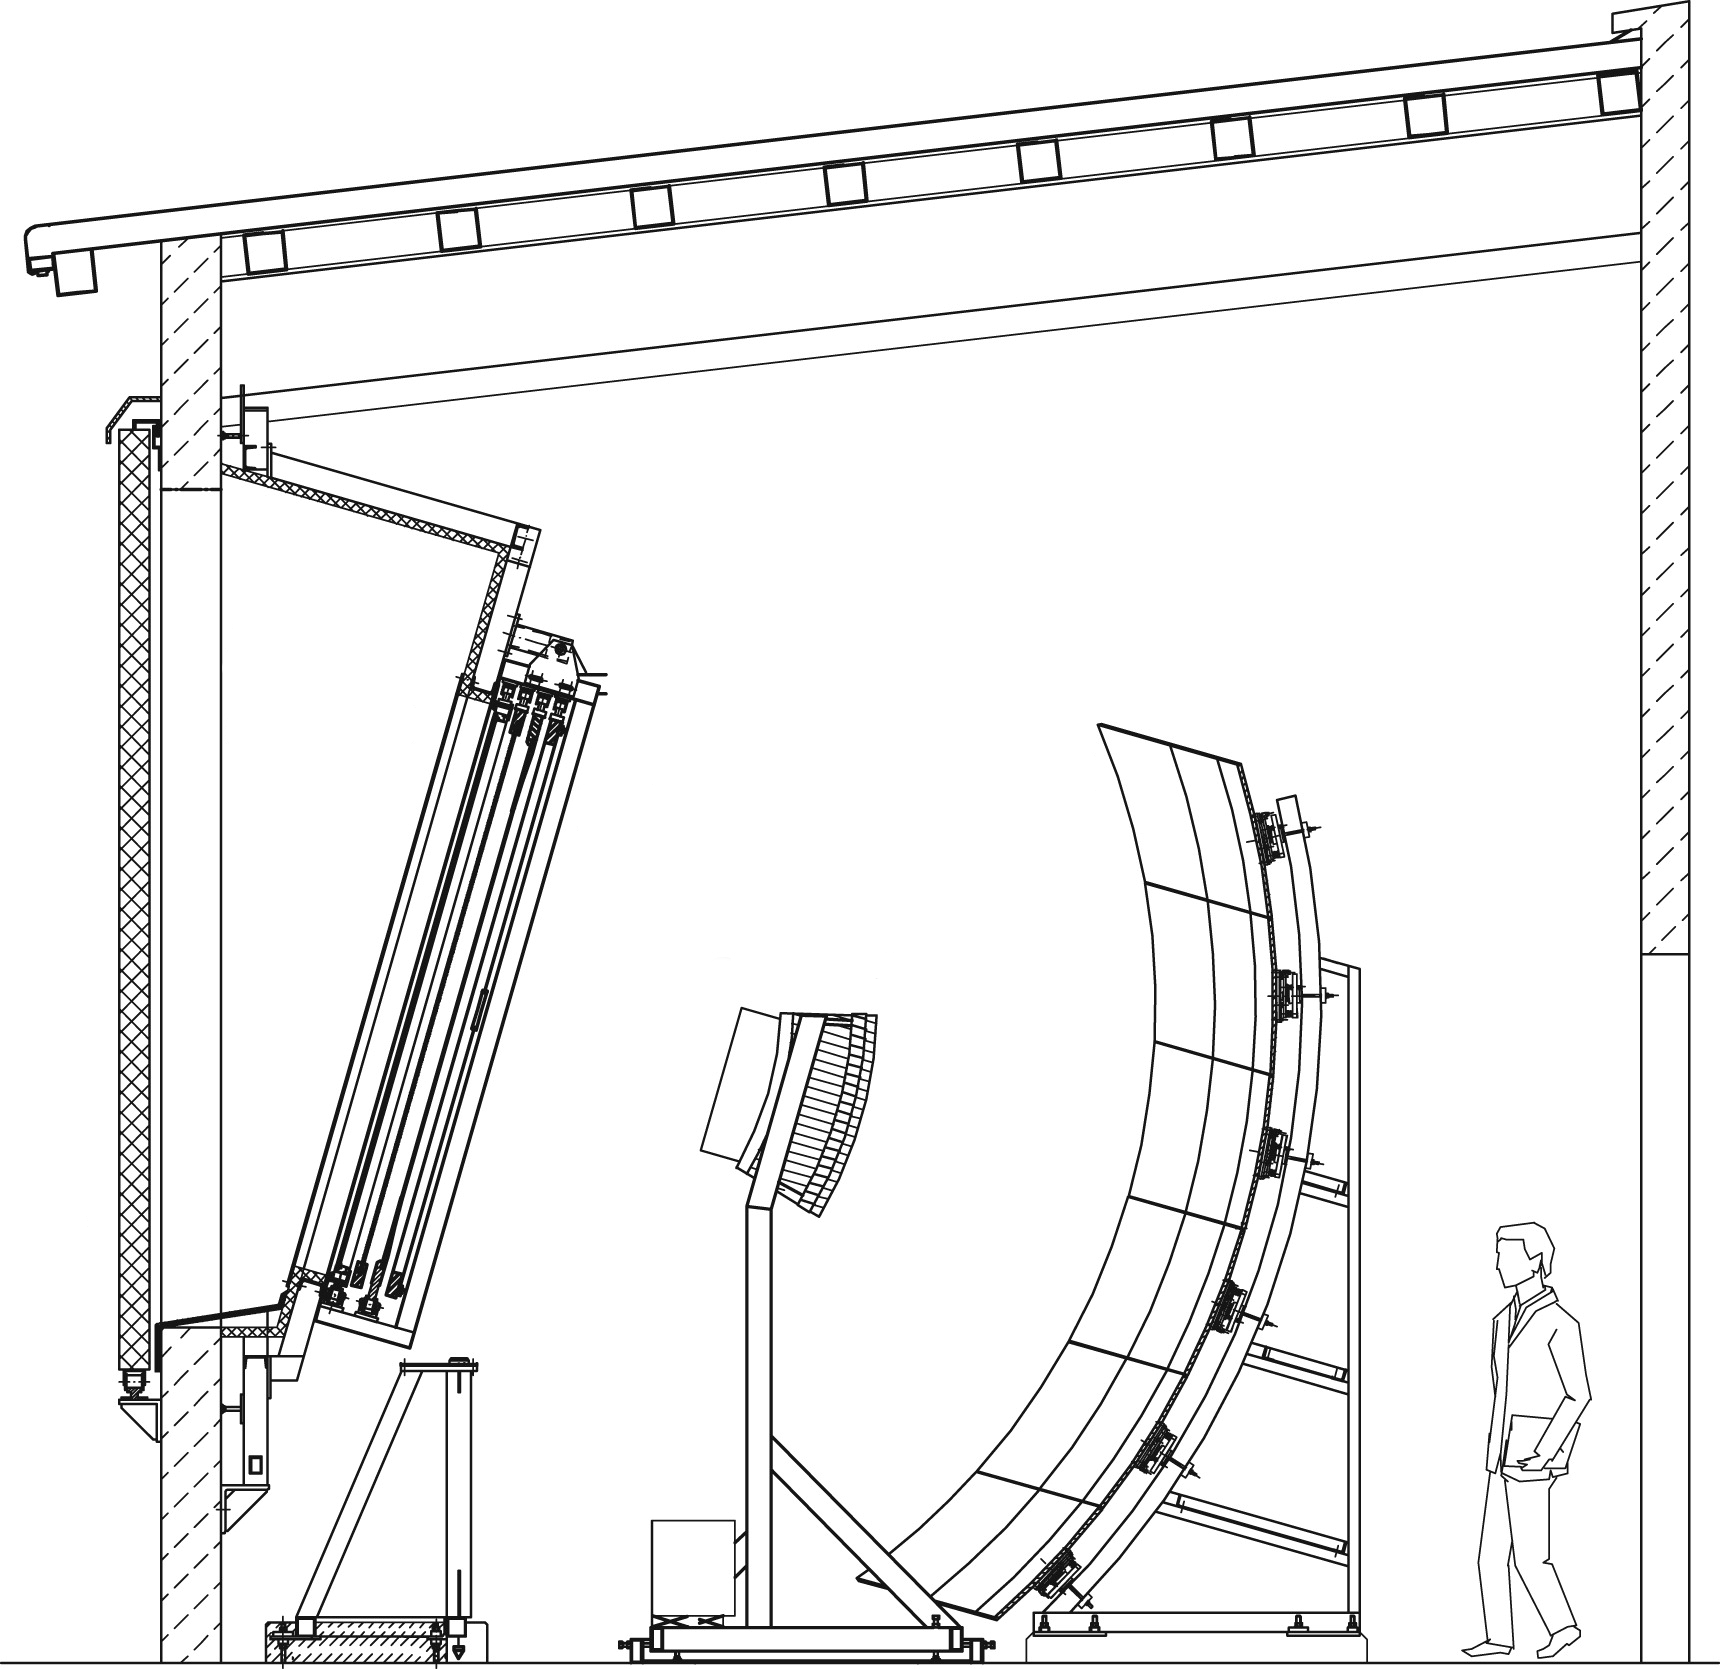
\includegraphics[height=0.45\textwidth]{auger-observatory/fd_schematic.png}
  \label{fig:fd-schematic}
  }
  \caption[]{\subref{fig:auger-map} Overview of the \PAO and its' detector 
  components. The black dots mark the placement of \WCDs in the \SD. The blue 
  lines indicate the location and \FOV of the \FDs. \HEAT (red) and \CO overlook 
  the SD-750 Infill area, where a denser spacing of stations separated by 
  \SI{750}{\meter} complement the SD-1500 main array. From 
  \cite{vebericIndexHttpWebiapkitedu}. \subref{fig:fd-schematic} Cross section 
  of the components of a single telescope, located in an \FD building, modified 
  from \cite{abrahamFluorescenceDetectorPierre2010}.}
  \label{fig:pao-images}
\end{figure}


\subsection{Optical System}
\label{ssec:fd-design}

The \FD telescopes are designed following the schematic of a Schmidt camera with
corrector plates. The individual components located on the optical axis are, in 
the order that light traverses them (see \cref{fig:fd-schematic}, 
\cref{fig:fd-inside-view} and \cite{abrahamFluorescenceDetectorPierre2010}):

\begin{enumerate}[label=(\Alph*)]
  \item \textbf{The shutter}, which consists of two massive metal doors, shields
  the aperture from atmospheric influences such as strong winds or rain. It also
  serves as a light shield that protects the sensitive camera electronics during
  the day.

  \item A \textbf{MUG6 \UV Filter} is installed in the light path in order to 
  block visible light from entering the telescope. It separates the climate 
  controlled inside of the \FD buildings from the outside via a circular
  aperture that measures \SI{2.2}{\meter} in diameter. 
  
  \item \textbf{Corrector lenses} are located in a ring around the edge of the 
  aperture. The ring has an inside diameter of \SI{1.7}{\meter} and manages to 
  increase the light collection area, while minimizing spherical aberrations in 
  the camera.

  \item \textbf{The curtain} curtain provides a secondary failsafe that prevents
  high-intensity light from reaching the sensitive electronics. The curtain 
  sits outside of the light path, but can be deployed in emergency situations, 
  or during daytime work and maintenance.

  \item \textbf{The mirrors} are a set of 60 hexagonal glass segments (36 square
  segments from anodized aluminum in the case of \LL and \LM) aligned in a 
  concave $\SI{3.6}{\meter}\times\SI{3.6}{\meter}$ shape, which reflects and 
  concentrates incoming light towards the camera.

  \item For \textbf{the Camera} refer to the next subsection.
\end{enumerate}

\subsubsection{\acf{HEAT}}
\label{sssec:HEAT}

The fifth and newest \FD-site, the \acl{HEAT} commissioned 2009, is located 
close to \CO, and looks out over the SD-750 array with three fluorescence 
telescopes. The setup of the optical system is (conceptually) identical to that 
of the standard \FD-sites. However, in the case of \HEAT, the entire telescope 
building can be rotated upwards by $30^\circ$. This allows the observation of 
the upper atmosphere, where lower energy \EASs are more prevalent. \HEAT extends
the energy scale seen by the \FD by one order of magnitude 
\cite{mathesHEATTelescopesPierre2011}.

\subsection{Camera and Readout Electronics}

The camera for each telescope consists of 440 Photonis XP3062 \PMTs that serve 
as the individual pixels. The specific model is chosen because it minimizes 
afterpulsing in the anode trace, and has a reasonable quantum efficiency 
($\approx30\%$) at the target wavelength (\SIrange{350}{400}{\nano\meter}) that 
the \FD monitors \cite{xiaoCalibrationPhotonisXP30622005}. The \PMTs are 
arranged in 22 rows and 20 columns. Each pixel has a solid angle acceptance of 
$\Omega = \SI{5.94e-4}{\sr}$. Reflective star shapes with threefold symmetry 
sit between neighbouring pixels to boost light collection efficiency, as well as
increase the camera point resolution. Finally, the voltage at the anode of the 
\PMTs is read out at a sampling frequency of \SI{10}{\mega\hertz} 
(\SI{20}{\mega\hertz} for \HEAT) and digitized by 12-bit \ADC-converter stages. 

The accurate reconstruction of an \EAS requires the camera to have an excellent 
background rejection (of e.g. transient stars in the camera \FOV). On top of 
this, signals must be processed quickly to keep a potential timing offset 
between \FD and \SD minimal, and enable a hybrid reconstruction. The \FD 
electronics achieve this via a simple, hierarchical trigger logic. A \FPGA 
scans the incoming signal from one column of pixels in a \FLT-stage. It 
calculates the running sum of the last 16 (baseline\footnote{calculated as the 
mean \ADC value over 65536 ($\cong\SI{6.554}{\milli\second}$) samples} 
subtracted) \ADC samples per pixel and compares the result to a reference 
threshold. If the sum exceeds the reference threshold a \FLT is issued and the 
pixel data is written to a \SRAM. This achieves two things. First, the number of
\FLTs over a period of time is used to calculate an \FLT rate per pixel. The 
reference threshold is updated according to this trigger rate, such that the 
\FLT matches a \SI{100}{\hertz} trigger rate. Secondly, the number of 
simultaneous \FLTs per column, or multiplicity, is evaluated and passed on to 
the \SLT-stage.

There, the active pixels (that have raised a trigger in the last 
\SI{100}{\nano\second}) are searched for spatial correlations. If a collection 
of at least 4 pixels are found whose layout corresponds to a set of predefined
masks a \SLT is issued. These predefined masks aim to identify straight tracks 
in the camera \FOV, and decrease the trigger rate from 
$\SI{100}{\hertz\per\mathrm{pixel}}$ in the \FLT to 
$\SIrange[range-units = single]{0.1}{10}{\hertz\per\mathrm{telescope}}$ in the 
\SLT. Following, a \TLT separates true air shower events from noise with 
$\approx94\%$ accuracy by performing a data-based cut on the multiplicity of 
active pixels \cite{abrahamFluorescenceDetectorPierre2010}. This reduces the 
trigger rate to $\SI{0.01}{\hertz\per\mathrm{telescope}}$. 

Finally, \TLTs from all telescopes in a building are analyzed for events that
pass the \FOV of multiple cameras, and an event level trigger, or T3, is issued
to the \CDAS at a rate of approximately 
$\SI{0.02}{\hertz\per\mathrm{building}}$.

\subsection{Telescope Calibration}
\label{ssec:fd-calibration}

The description of the event reconstruction in \cref{sec:event-reconstruction}
will reveal that in order to estimate the primary particle energy the number of
photons incident on the \FD-camera need to be known. This poses a big challenge.
While the camera signal response correlates with the number of photons observed
per \EAS, the correlation coefficient is completely determined by the gain of 
the telescope readout electronics, which need not be constant. It has been shown
that the camera response to the same signal can change by up to $6\%$ under 
suboptimal conditions \cite{filipJumpsXYCalibration2024}.

To account for this, the \PMTs need to be calibrated on a nightly basis. During
calibration the camera is exposed to a lightsource of known radiance, and the 
camera response (in units of \ADC) is logged. Tying all information together, 
this allows the calculation of (absolute) pixel calibration constants, 
$C^\mathrm{pixel}_\mathrm{abs.}$, in units of \SI{}{$\gamma$\per\ADC}. It is
imperative that these quantities are measured with high precision, as
uncertainties on $C^\mathrm{pixel}_\mathrm{abs.}$ contribute linearly to the 
uncertainty of the reconstructed primary particle energy. Currently, the pixel
calibration constants are measured with an uncertainty of approximately $9\%$
\cite{dawsonUpdateAugerEnergy13}. This represents the biggest contribution to 
the total uncertainty in the \PAO energy scale of $14\%$ 
\cite{verziEnergyScalePierre2013}.

\subsubsection{Atmospheric laser shots}

The \PAO operates two atmospheric lasers, the \CLF, and the \XLF 
\cite{collaborationTechniquesMeasuringAerosol2013}. Their primary science case 
is monitoring atmospheric conditions in order to model the development of \EASs
accurately. The two instruments provide vertical laser beams with stable power,
that, due to their very narrow frequency spectrum, translate to a stable
output of photons. In theory, the number of photons that scatter off of air 
molecules and hit the \FD-cameras per laser pulse is calculable. Analyzing the
telescope response to these laser pulses allow for an absolute calibration of 
\FD-\PMTs. In practice this proves impractical however. The air conditions in 
the atmosphere are not known with sufficient precision. Moreover, not all
pixels in all telescopes see the laser beams, which drastically lowers the 
accuracy of the presented method.

\subsubsection{Drone based calibration}

A remote-controlled drone equipped with a light source is used to simulate a 
distant point source in the \FD-\FOV \cite{wernerDesignTestFlying2010, 
tomankovaOpticalPropertiesCalibration2016}. In principle the hardware can be
used to calibrate the individual pixels of a camera, as the source radiance is
known. In practice the drone based approach takes a long time to illuminate 
every pixel. Other methods are less time intensive and therefore preferred. 
Nevertheless, the drone proves useful in measuring the optical properties of 
the \FD-mirrors, such as the \PSF.

\subsubsection{Drum calibration}

\begin{figure}[t]
  \centering
  \subfloat[]{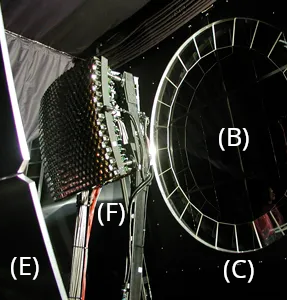
\includegraphics[height=0.32\textwidth]{auger-observatory/fd_camera.png}
  \label{fig:fd-inside-view}
  }\hspace{0.1cm}
  \subfloat[]{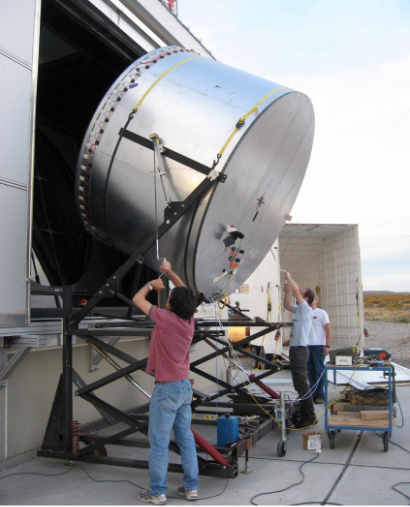
\includegraphics[height=0.32\textwidth]{auger-observatory/drum_mounting.png}
  \label{fig:drum-mounting}
  }\hspace{0.1cm}
  \subfloat[]{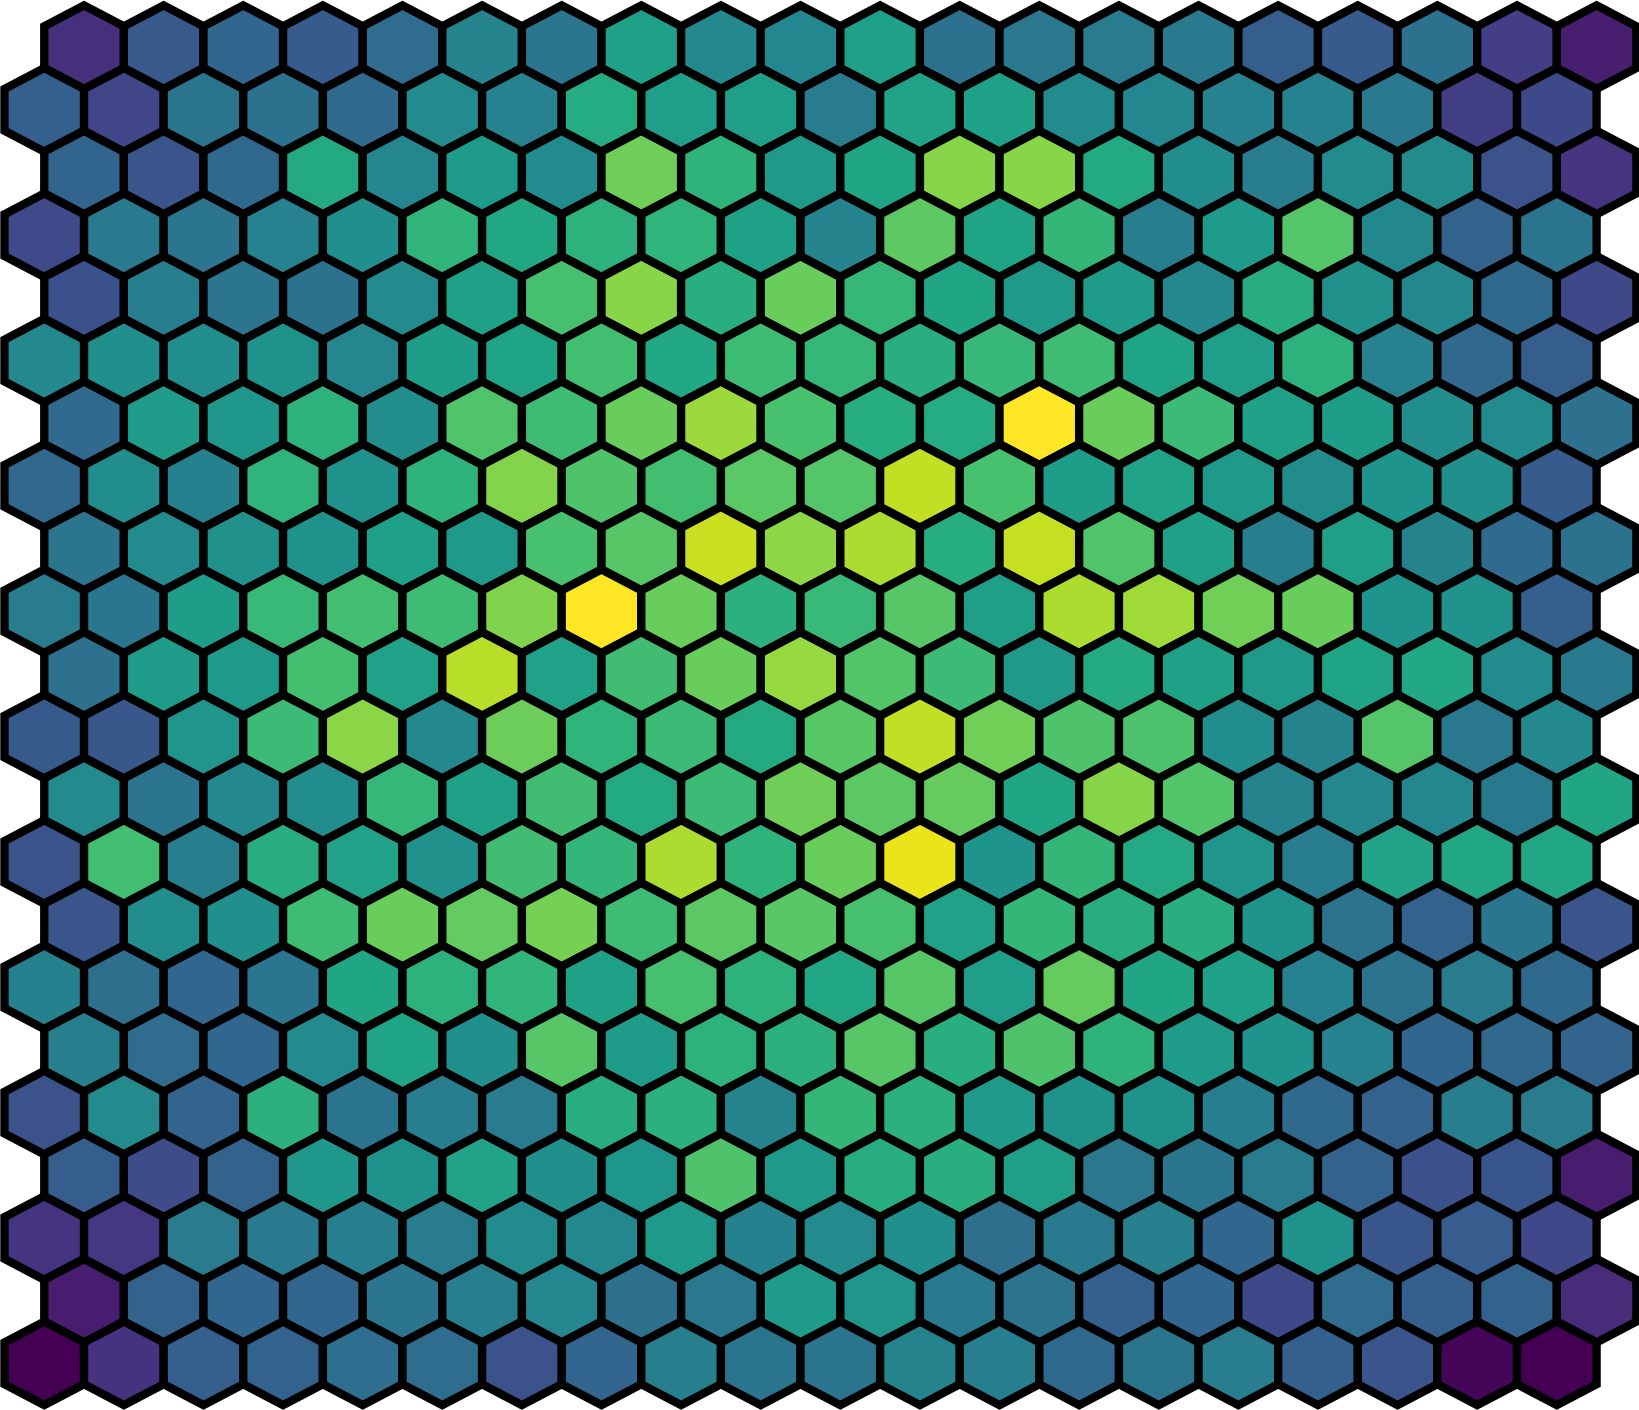
\includegraphics[height=0.32\textwidth]{auger-observatory/cal_a_response.png}
  \label{fig:cal-a-example-response}
  }
  \caption[]{\subref{fig:fd-inside-view} View of the inside of an \FD-telescope.
  The different detector components are labelled and described in more detail in
  \cref{ssec:fd-design}. Picture from \cite{pierreaugerobservatoryP22500022004} 
  \subref{fig:drum-mounting} The drum light source is mounted in front of the 
  aperture of a telescope at \CO for an absolute calibration. From 
  \cite{crissUpdateRecentAbsolute2010}. \subref{fig:cal-a-example-response} The 
  integral signal per pixel received by the camera in bay 2 of \CO for a 
  relative calibration measurement (cal. A) before standard \DAQ on 2024-11-20.}
  \label{fig:camera-stuff}
\end{figure}

The absolute calibration method currently in use at the \PAO is the drum 
calibration. The name derives from the shape of the light source, visible in 
\cref{fig:drum-mounting}. It is a cylinder with a diameter of \SI{2.5}{\meter} 
and depth of \SI{1.4}{\meter} with two NSHU550 \UV \LEDs installed at its' 
center. A reflective laminate uniformly distributes the light from the \LED over
the interior of the drum \cite{brackAbsolutePhotometricCalibration2004}. The 
radiance of the lightsource is carefully measured before, during, and after 
every \DAQ campaign \cite{brackAugerFluorescenceDetector2013}. To measure 
$C^\mathrm{pixel}_\mathrm{abs.}$ via the drum lightsource the cylinder frame has
to be mounted on top of the \FD aperture. Once done, all pixels in the telescope
camera are illuminated simultaneously with a single \LED pulse and the signal
response can be read out.

While the measurement itself is quick it requires time, manpower, and knowledge
to set up. For this reason the last absolute calibration of the \FD-telescopes 
with the drum lightsource has been conducted more than ten years ago in 2013 
\cite{dorofeevFDAbsoluteCalibration2013}. 

\subsubsection{Calibration A, B and C}

In order to address the lack of a nightly absolute calibration relative 
calibration systems exists to track the telescope evolution over time. These 
relative calibration systems are a set of \LCUs and identical for each building
\footnote{\HEAT has one copy for each of its' telescopes}.
They consist of three central \LED light source and optical fibers that 
transport photon signals to diffusers located at three different exit ports at 
the six different telescopes \cite{robertsCalibrationPierreAuger2003}. The 
location of the exit ports are as follows:

\begin{enumerate}[label=(\Alph*)]
	\item In the center of the mirror, directly illuminating the \FD-camera.
	\item Above the camera body, illuminating the pixels indirectly via the 
	mirror.
	\item Outside the \FD building and pointed towards the shutter.
	Reflective liners on the inside of the shutter redirect the light into 
	the aperture and eventually the camera.
\end{enumerate}

In principle, the combination of Calibration A, B, and C allow to monitor the 
aging of the different detector components, and provide an end-to-end 
calibration, in which the whole optical system of the telescopes is probed. Only
Calibration A is performed to track changes in the pixel-\PMTs in practice. The 
remaining telescope constituents have been shown to be stable over the timespan 
of years \cite{brackAugerFluorescenceDetector2013, 
dorofeevFDAbsoluteCalibration2013}.

Two Calibration A measurements are performed during each night. One before the 
start of \DAQ, and one after the data-taking ends. During the measurement the 
\LED emits 50 light pulses with a duration of $\approx\SI{60}{\micro\second}$ at
a wavelength of \SI{470\pm25}{\nano\meter} \cite{menshikovLEDCalibrationUnit}. 
The optical signal is guided through six cables to the diffusers at the center 
of the mirror. A seventh fiber feeds the light back to the \LCU, where a
photodiode digitizes the signal $S_\mathrm{LCU}$. The readout of pixel-data is 
forced via an external trigger coincident with every light pulse. The overall
signal recorded in the \FD time trace from the calibration light pulse(s),
$S_\mathrm{CalA}$, can be recovered by first estimating and subtracting the 
trace baseline \cite{schaferReconstructionBaselineUndershoot2022}, determining 
the pulse start and stop via a pulse-finding algorithm (see \todo{xy section 
ref here}), and summing the \ADC bins within the pulse-window. 
\cref{fig:cal-a-example-response} shows example data analyzed in this fashion. 
From $S_\mathrm{LCU}$ and $S_\mathrm{CalA}$ the calibration constants measured 
in a reference night via calibration method $i$ can be forward- or 
backpropagated to an arbitrary point in time according to 
\cite{salinaNewCalibrationTask2014, salinaAnalisiDatiXY2025} like

\begin{equation}
\label{eq:cal-a-propagation}
C^{\mathrm{pixel},\,i}_{\mathrm{abs.}} = C^{\mathrm{pixel},\,i}_{\mathrm{abs.},\,\mathrm{ref}}\,\cdot\,\frac{S_\mathrm{LCU}}{S_\mathrm{LCU}^\mathrm{ref.}}\,\frac{S_\mathrm{CalA}^\mathrm{ref.}}{S_\mathrm{CalA}}\,c_\mathrm{LCU}^\mathrm{Corr.}\,c^\mathrm{Corr.}_\mathrm{Halo}.
\end{equation}

In \cref{eq:cal-a-propagation} the two factors $c^\mathrm{Corr.}_i$ give 
different corrections to the end result that need to be considered. First, a 
time-dependant factor $c^\mathrm{Corr.}_\mathrm{LCU}$ absorbs the change of 
radiance in the \LCU \LED after a replacement in 2011/2012 took place in all 
telescopes \cite{menshikovLEDCalibrationUnit}. A second factor accounts for the 
fact that not all photons that hit the camera body are registered in the \PMTs. 
Some light is reflected away, and does not contribute to the absolute 
calibration. Consequently, $C^{\mathrm{pixel},\,i}_\mathrm{abs.}$ would be 
underestimated without a correction factor $c^\mathrm{Corr.}_\mathrm{Halo}$ 
\cite{brackFluorescenceDetectorAbsolute13}.

\subsubsection{XY Scanner}

The XY-Scanner is a novel end-to-end calibration method that aims to be the
successor of the drum calibration system \cite{engelNewEndtoendCalibration2017}.
It consists of a portable \IS lightsource mounted on an XY translation stage. 
Instead of illuminating the entire aperture with a single flash of a big 
lightsource, the XY-Scanner fires many flashes from different positions in the 
aperture. This compromises measurement time for much easier handling and better
systematics on the resulting pixel calibration constants. The setup and analysis
of the method are summarized in \todo{xy scanner chapter here}, and described in
detail in \cite{schaferXYScannerVersatileMethod2023}

\section{The Surface Detector (SD)}
\label{sec:sd}

The \acf{SD} are a collection of more than 1660 stations spread in a regular 
pattern over the surface of the Pampa Amarilla. The position of each station is 
shown in \cref{fig:auger-map}. Each station is equipped with hardware that 
offers several detection channels to ionizing particles on the ground. Their 
remote location complicates maintenance work and the transfer of measurement 
data. For this reason the stations are operating largely autonomously, only 
communicating essential information to the \CDAS (see \cref{sec:cdas}). They 
derive their electrical power from a solar panel, and have (limited) 
computational resources at hand that control communication with the \CDAS, data 
readout, and run procedures to self-calibrate the individual detectors. 

\subsection{Station components}
\label{ssec:station-components}

The main detector and processing components (\WCD, \UUB, etc.) are presented in
the following subsections. Some auxiliary hardware components (auxiliary in the 
context of this work, not the function of the stations) are only briefly 
mentioned here:

\begin{itemize}
	\item Two $\SI{55}{\watt}_\mathrm{peak}$ solar panels provide 
	electricity during solar periods 
	\cite{collaborationPierreAugerObservatory2016}.
	\item Two \SI{105}{\ampere\hour} batteries deliver power during	the 
	dark \cite{collaborationPierreAugerObservatory2016}.
	\item A Motorola Oncore UT+ \GPS-receiver determines the position of the
	station using a pulse precision of \SI{5}{\nano\second} 
	\cite{networktimefoundationMotorolaOncoreGPS, 
	collaborationPierreAugerObservatory2016} ($\cong\SI{1.5}{\meter}$
	position accuracy).
	\item A commercial \SI{12}{\dBi} Yagi antenna \cite{rfwel12DBiYagi} 
	establishes communication with the \CDAS.
\end{itemize}

\subsubsection{\acf{WCD}}

\begin{figure}[t]
  \centering
  \subfloat[]{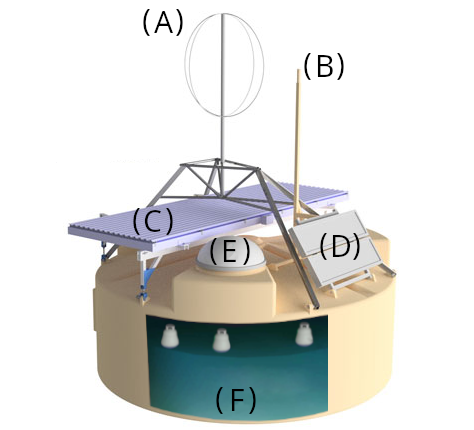
\includegraphics[height=0.37\textwidth]{auger-observatory/sd_station.png}
  \label{fig:sd-station-render}
  }\hspace{0.2cm}
  \subfloat[]{\includegraphics[height=0.37\textwidth]{auger-observatory/SSD_high_contrast.png}
  \label{fig:ssd-high-contrast}
  }
  \caption[]{\subref{fig:sd-station-render} A model of an \SD-station, showing
  wht the label (A) the \RD, (B) the comms antenna, (C) the \SSD, (D) the solar
  panels, (E) the electronics box containing the \UUB, and (F) the inside of the
  \WCD with the three \LPMTs. Adopted with changes from 
  \cite{filipPotentialNeuralNetwork2023}. \subref{fig:ssd-high-contrast} The 
  \SSD without enclosing box, showing the individual scintillator strips and 
  \WLSs. From \cite{schmidtUHECR2024ProceedingEdits25}.}
  \label{fig:sd-station-components}
\end{figure}

The \acf{WCD} is the main detector component, and common to all \SD-stations 
since the construction of the \PAO began. It is an oblate cylinder with a 
diameter of \SI{3.6}{\meter} and height of $\SI{1.2}{\meter}$ as seen in 
\cref{fig:sd-station-render}. The interior is filled with a sealed liner 
containing \SI{12000}{\liter} of filtered water, and shielded from exterior 
light via a polyethylene housing \cite{allekotteSurfaceDetectorSystem2008}. The 
darkness in the cylinder is occasionally interrupted by flashes of light 
stemming from relativistic particles producing Cherenkov radiation in the water.
This light bounces off of the reflective interior walls until it reaches one of 
three identical \SI{230}{\milli\meter} Photonis XP1805 \LPMTs 
\cite{tripathiSystematicStudyLarge2003} that are optically coupled to the inside
volume of the liner.

The \WCD needs to be able to accurately reconstruct a large dynamic range of
signals, starting from individual particles to $>10^3$ muons entering the water
\cite{abrahamTriggerApertureSurface2010a}. To achieve this, the \LPMTs 
characteristics are monitored by two channels, the \HG and the \LG. The \LG 
is connected directly to the dynode of the \PMTs, whereas the \HG tracks the 
anode voltage. The \HG-channel is thus amplified to have a gain ratio of 
$\sim32$. Both channels are read out via 12-bit AD9628 \FADCs 
\cite{analogdevicesinc.AD9628DatasheetProduct2015} at a sampling rate of \SI{120}{\mega\hertz} (corresponding to a binning of \SI{8.333}{\nano\second}). 

A fourth, \SI{25}{\milli\meter} \SPMT of type Hamamatsu R8619 
\cite{hamamatsuphotonicsPhotomultiplierTubeR8619} is installed near the center
of the tank. It is exposed to less light due to its relatively small size, and 
extends the dynamic range of the \WCD to about \SI{20000}{\VEM}.

\subsubsection{Calibration}

The same considerations as in \cref{ssec:fd-calibration} apply to the data
recorded by the \WCD (and all other \SD components). The detector information 
needs to be put into a physical context in order to be interpreted correctly.
For the particle detectors at the \PAO (\WCD, \SSD, and \UMD) this context is 
given by atmospheric muons, as they have a characteristic energy deposit and 
signature in the active medium. The measurement data (in units of \ADC) is
converted to the quantity of muons (or \MIPs, in the case of the \SSD) that
would be needed to be injected vertically\footnote{To absorb dependencies of the
track length in the detector} in the detector to record the same signal 
strenght. This, for the \WCD, gives raise to two quantities that need to be 
tracked in order to provide calibrated data:

\begin{itemize}
	\item \Ivem is the most probable pulse height (in units of \ADC) 
	recorded by the \WCD \PMTs when a muon passes vertically through the 
	center of the water volume.
	\item \Qvem gives the most probable value (measured in \ADC as well) for
	the integral of the muon pulse, corresponding to the energy deposited in 	the detector by the particle.
\end{itemize}

The trigger thresholds (compare \cref{ssec:sd-triggers}) in the \WCD are set in
terms of \Ivem. For this reason, the stations operate a self-calibration
algorithm that delivers a rate-based estimate of \Ivem, called \VemOnline that 
is accurate to within $\sim5-10\%$ \cite{bertouCalibrationSurfaceArray2006} of 
the true value of \Ivem.

The value of \VemOnline is adjusted by a simple and robust algorithm. It employs
a calibration trigger that requires a coincident signal of at least 
\SI{1.75}{\VemOnline} in all three \LPMTs. In the case of one or more tubes
being broken the trigger thresholds are adjusted in order to ensure the stable 
operation of the remaining \PMTs 
\cite{convengaLocalStationCalibrationDummies2023}.

An additional cut of \SI{2.5}{\VemOnline} is applied per \LPMT, and the number 
of triggers during a timespan measuring at most \SI{60}{\second} is tracked. If
the trigger rate of the calibration trigger exceeds a target rate of 
\SI{72}{\hertz} during this period, the value of \VemOnline is increased. This 
results in more stringent trigger conditions, and will decrease the trigger rate
during the following \DAQ period. Similarly, the value of \VemOnline is 
decreased if the calibration trigger rate is lower than \SI{68}{\hertz}. If the 
trigger rate lies within \SI{70\pm2}{\hertz} the \DAQ period is increased 
(beginning with \SI{10}{\second}) by \SI{5}{\second} to limit the influence of 
Poissonian noise on the estimate \cite{bertouCalibrationSurfaceArray2006, 
convengaLocalStationCalibrationDummies2023}.

\subsubsection{\acf{SSD}}

\subsubsection{\acf{UMD}}

\subsubsection{\acf{RD}}










\subsubsection{\acf{UUB}}

\begin{figure}[t]
  \centering
  \subfloat[]{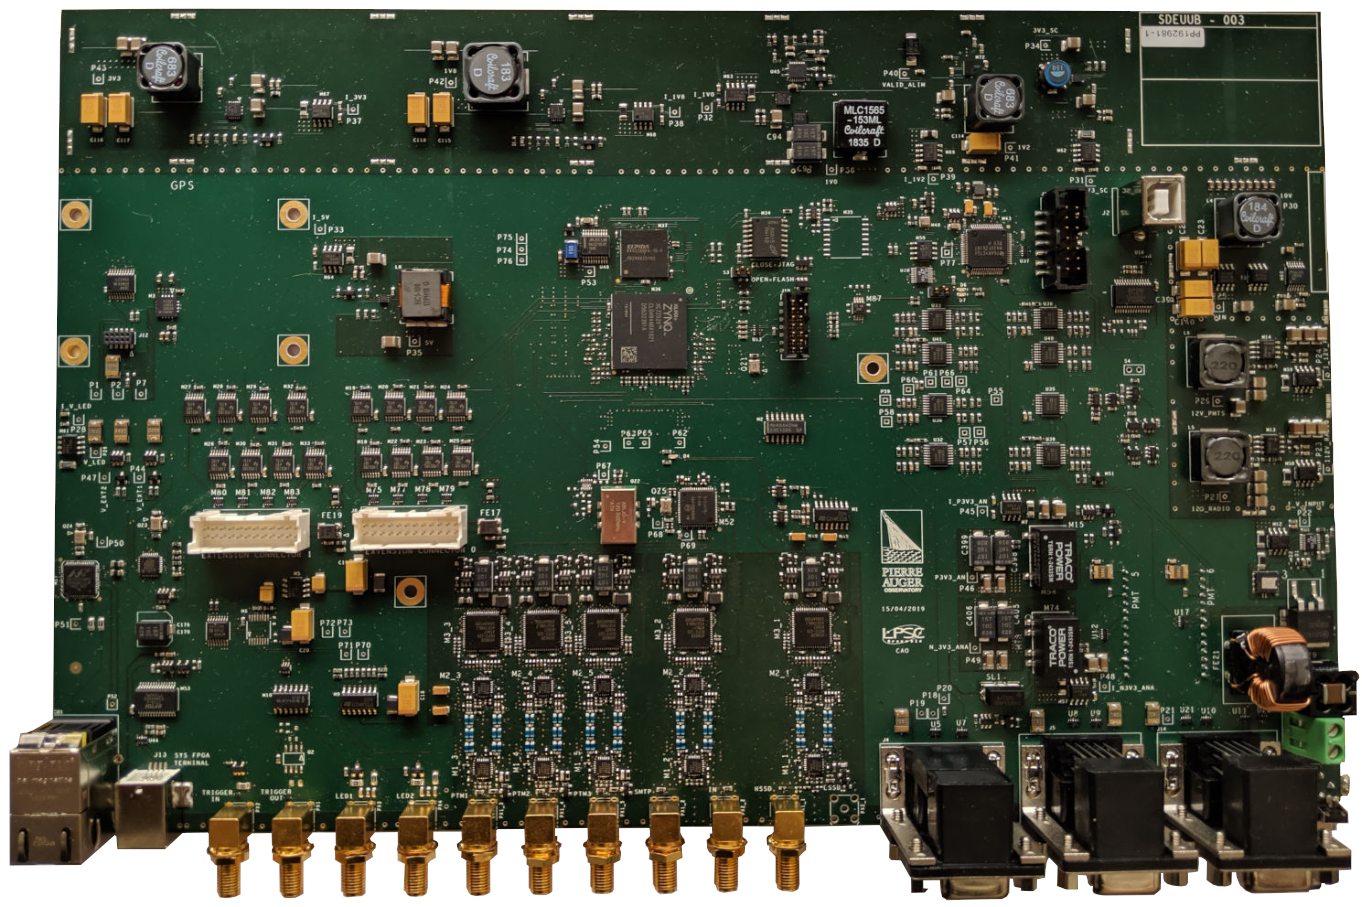
\includegraphics[height=0.42\textwidth]{auger-observatory/uub_annotated.png}
  \label{fig:uub-pcb-board}
  }\hspace{0.2cm}
  \subfloat[]{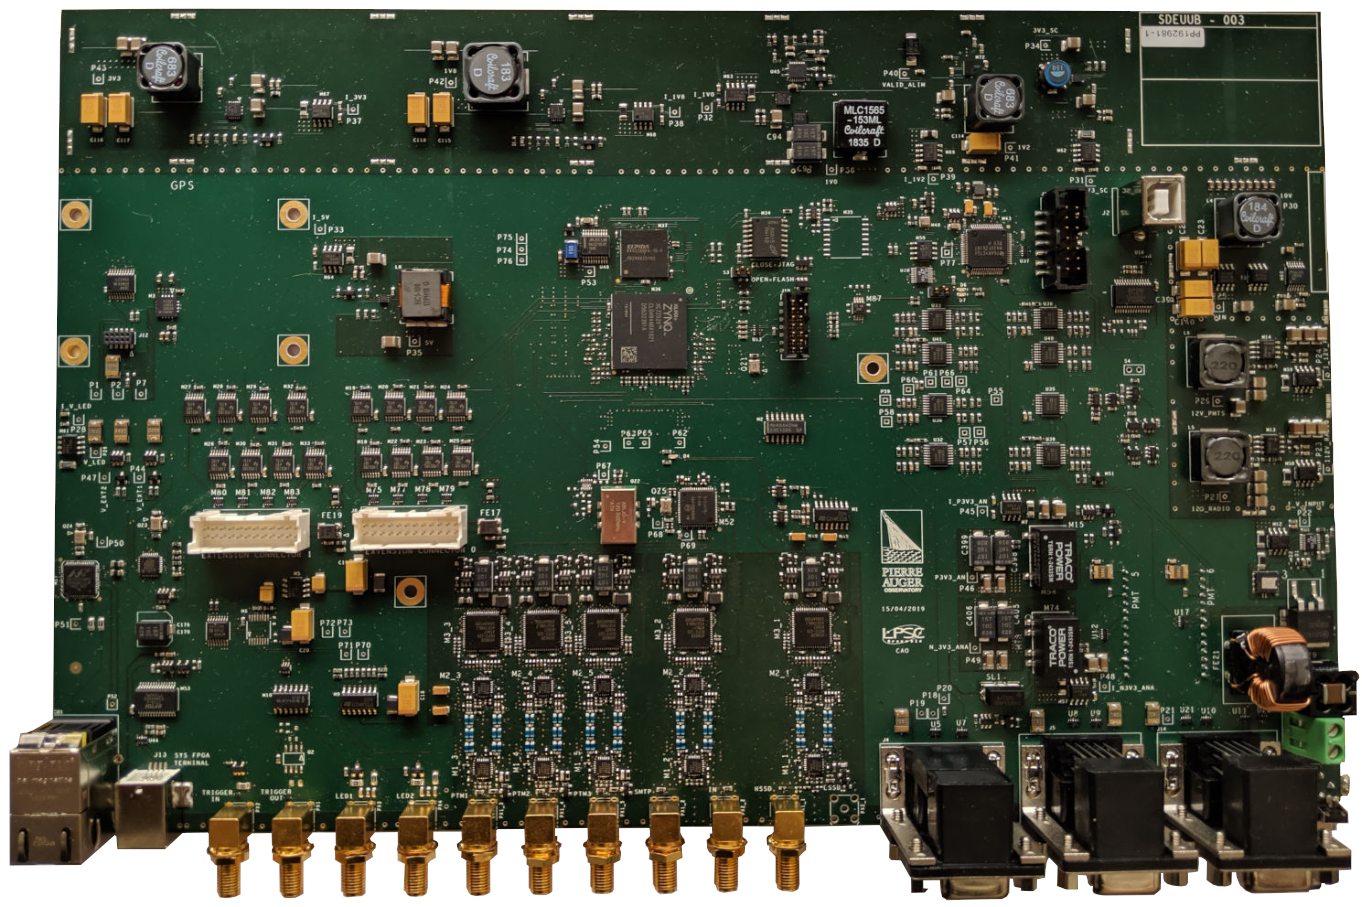
\includegraphics[height=0.42\textwidth]{auger-observatory/uub_annotated.png}
  \label{fig:uub-operative-logic}
  }
  \caption[]{\subref{fig:uub-pcb-board} . Image edited from \cite{nitzNewElectronicsSurface2021} \subref{fig:uub-operative-logic} }
  \label{fig:uub-specifications}
\end{figure}

The \UUB, replacing the \UB in the AugerPrime detector upgrade, hosts all main 
electronic readout components of the station 
\cite{collaborationPierreAugerObservatory2016}. Most importantly, this includes 
an Artix-7 \FPGA \cite{xilinx7SeriesFPGAs2020} for low-level signal processing,
as well as a Xilinx Zynq-7020 \SOC \cite{amdZynq7000SoC2023} that handles the 
front-end electronics and higher-level procedures.

\cref{fig:uub-pcb-board} and \cref{fig:uub-circuit-diagram} show the design and
architecture of the \UUB \PCB board respectively.

\todo{continue}

\subsection{Array structure}
\label{ssec:array-structure}

The \SD is designed to detect the footprint of an \EAS on the surface of the 
Earth. The choice of a detector segmented into many different sub-components is
deliberate. Operating a detector with a continous active region is impractical, 
as \EASs can reach many kilometers in extent. It is sufficient to probe the 
shower footprint at select few positions and reconstruct the \EAS from this 
limited knowledge. As already realized by Pierre Auger, the separation between 
sampling points influences the types of air showers that can be detected 
\todo{ref here}. The lower the separation, the more low-energy \EAS become 
observable.

Already before the construction of the \PAO it was decided that the \SD will 
host sub-arrays of different sizes and separations 
\cite{watsonDevelopmentPierreAuger}. This ensures that the observatory can 
make accurate measurements of \EAS over many decades of energy. 
\cref{tab:sub-array-details} lists the most important characteristics of the 
individual sub-arrays. In all of them, the stations are arranged on a grid of 
isoceles triangles. The SD-1500, or main array, is the largest of the three 
existing grids. It is currently the detector with the highest accumulated 
exposure to \CRs worldwide \cite{aabPierreAugerObservatory2020}.

Inset in the north-west of the SD-1500 are the SD-750 (Infill), and SD-433
(compare \cref{fig:auger-map}). Their vicinity to \CO and \HEAT ensure that the 
hybrid reconstruction (see \cref{sec:event-reconstruction}) of \EAS remain 
possible also for energies below \SI{1e17}{\eV}
\cite{mathesHEATTelescopesPierre2011}. Contained within both arrays are several 
\RND environments, such as the \AERA \cite{fuchsAugerEngineeringRadio2012}, or 
IceCube@Auger \cite{schroederIceTopAuger2025}. 

The Infill is also home to doublet and triplet detectors, where two \SD-stations
(with e.g. different electronics) are installed at the same site. They are used 
to study timing offsets and (un)certainties, as well as verify the correct 
operation of the upgraded AugerPrime electronics 
\cite{payerasCompatibilityUBUUB2023}.

\begingroup
\renewcommand{\arraystretch}{1.0}
\begin{table}
	\begin{center}
	\caption{Characteristics of the different \SD sub-arrays}
	\begin{tabular*}{1.0\textwidth}{@{\extracolsep{\fill}} l|ccccl}
  \toprule
	\hline
	Array & Sep. & Stations & Area & full efficiency\tablefootnote{The full
	efficiency gives the minimum energy for which the detection of the \EAS 
	is guaranteed.} & 
	Station components \\
	\hline
	\textbf{SD-1500} & \SI{1500}{\meter} & 1669 & 
	\SI{3000}{\kilo\meter\squared} & 
	\SI{3e18}{\eV} \cite{abrahamTriggerApertureSurface2010} & \WCD, \SSD, 
	\RD \\
	\textbf{SD-750} & \SI{750}{\meter} & 61 & \SI{25}{\kilo\meter\squared} &
	\SI{3e17}{\eV} \cite{fenuCosmicRayEnergy2023} & \WCD, \SSD, \RD, \UMD \\
	\textbf{SD-433} & \SI{433}{\meter} & 19 & \SI{2}{\kilo\meter\squared} &
	\SI{5e16}{\eV} \cite{silliPerformance433Surface2022a}\tablefootnote{for 
	hadronic primaries with $\theta < 45^\circ$} & \WCD, \SSD, \RD, \UMD \\
  \bottomrule
	\end{tabular*}
	\label{tab:sub-array-details}
	\end{center}
\end{table}
\endgroup

\section{Central Data Acquisition System (CDAS)}
\label{sec:cdas}

\section{Event detection and reconstruction}
\label{sec:event-reconstruction}

\subsection{\SD triggers and \EAS detection}
\label{ssec:sd-triggers}

\subsection{\FD triggers and \EAS detection}
\subsection{\Offline event reconstruction}
\todo{reconstructed quantities table}

